\documentclass[14pt,a4paper]{article}
\usepackage[a4paper, mag=1000, left=2cm, right=2cm, top=2cm, bottom=2cm, headsep=0.7cm, footskip=cm]{geometry}
\usepackage[utf8x]{inputenc}
\usepackage[T1,T2A]{fontenc}
\usepackage[english,russian]{babel}
\usepackage{indentfirst}
\usepackage[dvipsnames]{xcolor}
\usepackage[colorlinks]{hyperref}
\usepackage{listings} 
\usepackage{fancyhdr}
\usepackage{caption}
\usepackage{subfig}
\usepackage{color}
\usepackage{here}
\usepackage{array}
\usepackage{multirow}
\usepackage{subcaption}
\usepackage{amsmath}
\usepackage{latexsym}
\usepackage{graphicx}
\hypersetup{
	colorlinks = true,
	linkcolor  = black
}

\DeclareCaptionFont{white}{\color{white}} 

\sloppy

% Listing description

\usepackage{listings}
\usepackage{caption}
\DeclareCaptionFont{white}{\color{white}}
\DeclareCaptionFormat{listing}{\colorbox{gray}{\parbox{\dimexpr\textwidth-1.72\fboxsep\relax}{#1#2#3}}}
\captionsetup[lstlisting]{format=listing,labelfont=white,textfont=white,margin=0pt}
\lstset{language=C,
	basicstyle=\footnotesize,
	keepspaces=true,
	tabsize=4,               
	frame=single,                           % Single frame around code
	rulecolor=\color{black},
	captionpos=b,
	showstringspaces=false,	
	abovecaptionskip=-0.9pt,
	xleftmargin=3.4pt,
	xrightmargin=2.6pt,
	breaklines=true,
	postbreak=\raisebox{0ex}[0ex][0ex]{\ensuremath{\color{black}\hookrightarrow\space}},
	xleftmargin=3.2pt,
	literate={а}{{\selectfont\char224}}1
	{~}{{\textasciitilde}}1
	{б}{{\selectfont\char225}}1
	{в}{{\selectfont\char226}}1
	{г}{{\selectfont\char227}}1
	{д}{{\selectfont\char228}}1
	{е}{{\selectfont\char229}}1
	{ё}{{\"e}}1
	{ж}{{\selectfont\char230}}1
	{з}{{\selectfont\char231}}1
	{и}{{\selectfont\char232}}1
	{й}{{\selectfont\char233}}1
	{к}{{\selectfont\char234}}1
	{л}{{\selectfont\char235}}1
	{м}{{\selectfont\char236}}1
	{н}{{\selectfont\char237}}1
	{о}{{\selectfont\char238}}1
	{п}{{\selectfont\char239}}1
	{р}{{\selectfont\char240}}1
	{с}{{\selectfont\char241}}1
	{т}{{\selectfont\char242}}1
	{у}{{\selectfont\char243}}1
	{ф}{{\selectfont\char244}}1
	{х}{{\selectfont\char245}}1
	{ц}{{\selectfont\char246}}1
	{ч}{{\selectfont\char247}}1
	{ш}{{\selectfont\char248}}1
	{щ}{{\selectfont\char249}}1
	{ъ}{{\selectfont\char250}}1
	{ы}{{\selectfont\char251}}1
	{ь}{{\selectfont\char252}}1
	{э}{{\selectfont\char253}}1
	{ю}{{\selectfont\char254}}1
	{я}{{\selectfont\char255}}1
	{А}{{\selectfont\char192}}1
	{Б}{{\selectfont\char193}}1
	{В}{{\selectfont\char194}}1
	{Г}{{\selectfont\char195}}1
	{Д}{{\selectfont\char196}}1
	{Е}{{\selectfont\char197}}1
	{Ё}{{\"E}}1
	{Ж}{{\selectfont\char198}}1
	{З}{{\selectfont\char199}}1
	{И}{{\selectfont\char200}}1
	{Й}{{\selectfont\char201}}1
	{К}{{\selectfont\char202}}1
	{Л}{{\selectfont\char203}}1
	{М}{{\selectfont\char204}}1
	{Н}{{\selectfont\char205}}1
	{О}{{\selectfont\char206}}1
	{П}{{\selectfont\char207}}1
	{Р}{{\selectfont\char208}}1
	{С}{{\selectfont\char209}}1
	{Т}{{\selectfont\char210}}1
	{У}{{\selectfont\char211}}1
	{Ф}{{\selectfont\char212}}1
	{Х}{{\selectfont\char213}}1
	{Ц}{{\selectfont\char214}}1
	{Ч}{{\selectfont\char215}}1
	{Ш}{{\selectfont\char216}}1
	{Щ}{{\selectfont\char217}}1
	{Ъ}{{\selectfont\char218}}1
	{Ы}{{\selectfont\char219}}1
	{Ь}{{\selectfont\char220}}1
	{Э}{{\selectfont\char221}}1
	{Ю}{{\selectfont\char222}}1
	{Я}{{\selectfont\char223}}1,
	extendedchars=true
}

\DeclareCaptionFormat{hfillstart}{\hfill#1#2#3\par}
\captionsetup[table]{format=hfillstart,labelsep=newline,justification=centering,skip=-10pt,textfont=bf}


\usepackage{float}

\begin{document}

\begin{titlepage}
    \centering
    \textsc{Санкт-Петербургский политехнический университет Петра Великого}\\[3mm]
    \textsc{Институт компьютерных наук и технологий}\\[3mm]
    \textsc{Кафедра компьютерных систем и программных технологий}
	
	\vfill
	
	\textbf{Отчёт по лабораторной работе }\\[3mm]
	по курсу «Проектирование ОС и компонентов»\\[3mm]
	по теме «Драйвер символьного устройства»\\[41mm]
	
    \begin{flushright}
	\begin{minipage}{.35\textwidth}
		Выполнил студент гр. 13541/2:\\
		Волкова М. Д.\\[3mm]
		Проверил преподаватель:\\
		Душутина Е. В.
	\end{minipage}
    \end{flushright}
	
	\vfill

	Санкт-Петербург\\
	\the\year\ г.
\end{titlepage}


\renewcommand\contentsname{\centerline{Содержание}}
\tableofcontents
\newpage


\section{Цель работы}
\par Необходимо провести исследование библиотеки libusb на одной из операционных систем. Должен быть проведен анализ исходного кода и написано тестовое приложения для взаимодействие с usb устройством мыши или клавиатуры.

\subsection{Характеристики системы}
\begin{lstlisting}
osboxes@osboxes:~/Documents/study/os/listings$ cat /proc/version
Linux version 4.4.0-142-generic (buildd@lcy01-amd64-006) (gcc version 4.8.4 (Ubuntu 4.8.4-2ubuntu1~14.04.4) ) #168~14.04.1-Ubuntu SMP Sat Jan 19 11:26:28 UTC 2019

osboxes@osboxes:~/Documents/study/os/listings$ gcc --version
gcc (Ubuntu 4.8.4-2ubuntu1~14.04.4) 4.8.4
Copyright (C) 2013 Free Software Foundation, Inc.
This is free software; see the source for copying conditions.  There is NO
warranty; not even for MERCHANTABILITY or FITNESS FOR A PARTICULAR PURPOSE.

osboxes@osboxes:~/Documents/study/os/listings$ uname -a
Linux osboxes 4.4.0-142-generic #168~14.04.1-Ubuntu SMP Sat Jan 19 11:26:28 UTC 2019 x86_64 x86_64 x86_64 GNU/Linux

\end{lstlisting}

\section{Общее описание}

\par libusb - это библиотека C, которая предоставляет общий доступ к USB-устройствам. Она предназначена для использования разработчиками для облегчения производства приложений, взаимодействующих с USB-оборудованием.\\

\par Данная библиотеки поддерживает различные операционные системы: Linux, OS X, Windows, Windows CE, Android, OpenBSD/NetBSD, Haiku. Исследование данной библитеки будет происходить на версии для Linux, так как, например на Windows, ее функциональность несколько ограничена.\\

\par Для работы с USB устройством необходимо использовать драйвер.  Можно написать свой драйвер или использовать существующие драйвера ОС. Большинство USB устройств относятся к каким либо классам устройств. Для большинства таких типов устройств уже имеются драйвера в составе установленной ОС. Например, мышь относится к классу HID , для нее имеются стандартные драйвера в ОС. Через API, из своей программы обращаетесь к ОС, а она через драйвер к USB устройству. Но тогда создаваемое USB устройство должна поддерживать протокол HID. Это достаточно сложная надстройка над базовой функциональностью USB.\\

\par Для такого подхода можно использовать библиотеку libusb. Эта библиотека позволяет писать прикладные программы, напрямую обращающиеся к USB устройству, устраняя необходимость использования специальных драйверов ОС.\\

\par  В простейшем виде USB-устройство можно представить как некую древовидную структуру, включающую в себя «Конфигурации» (configurations), «Интерфейсы» (interfaces) и «Конечные точки» (endpoints).

\par «Конечная точка» устройства — это программная сущность, у которой есть свой уникальный идентификатор и которая может иметь буфер с некоторым числом байтов для приема-передачи информации. Но чтобы добраться до нее, приложению (под управлением хоста) нужно программным путем пройти через уровни «Устройства», «Конфигурации» и «Интерфейса». Каждый из них описывается стандартной программной структурой, и есть возможность выбирать, какие именно интерфейсы следует использовать, чтобы попасть в требуемую конечную точку.\\

\par Важная особенность USB — наличие только одного Мастера (ведущего), которым обычно является компьютер. Само USB-устройство всегда отвечает на разные запросы компьютера, о чем бы ни шла речь и в какую бы сторону ни передавалась информация.\\

\par Разработчик может написать полноценный драйвер для работы со своим USB-устройством, применяя уже имеющийся в системе заголовочный файл linux/usb.h.\\

\par Дело в том, что большинство низкоуровневых задач в Linux уже решены, и любая написанная программа будет иметь прикладной характер, хотя формально и получит название драйвера. Справедливо также заметить, что с каждой новой версией ядра Linux работа с USB становится проще.

\par Драйвер, написанный для поддержки USB-устройства, призван решать следующие задачи:

\begin{itemize}
    \item регистрация и удаление драйвера;
    \item регистрация и удаление устройства;
    \item обмен данными с устройством.
\end{itemize}

Но можно точно назвать один важный и естественный недостаток, который несет в себе программный модуль уровня драйвера, — платформенная непереносимость.

\par Однако, использование библиотеки libusb может устранить этот недостаток, так как:
\begin{itemize}
    \item используя единый кроссплатформенный API, она обеспечивает доступ к USB-устройствам в Linux, OS X, Windows, Android, OpenBSD и т.д.
    \item работает в пользовательском режиме: никаких специальных привилегий или прав не требуется, чтобы приложение взаимодействовало с устройством.
    \item не зависит от версии: поддерживаются все версии протокола USB, начиная с 1.0 до 3.1.
\end{itemize}

\section{Анализ библиотеки}

\subsection{Особенности библиотеки}
\begin{itemize}
    \item Поддерживаются все типы передачи (control/bulk/interrupt/isochronous)
    \item 2 интерфейса передачи: Синхронный (простой), Асинхронный (более сложный, но более мощный)
    \item Потокобезопасна
    \item Легковесна
    \item Поддержка горячего подключения
\end{itemize}

\subsection{API библиотеки}

\subsubsection{Устройства и дескрипторы устройств}
\par libusb имеет концепцию USB-устройства, представленного типом libusb\_device.Используя ссылку на устройство, вы можете определить определенную информацию об устройстве (например, вы можете прочитать данные дескриптора). \\

\par Функцию libusb\_get\_device\_list () можно использовать для получения списка устройств, подключенных в данный момент к системе. Это известно как обнаружение устройства.\\

\par Наличие ссылки на устройство, не означает, что оно обязательно будет использовано. Возможно, устройство было отключено от сети, может не быть разрешения на управление таким устройством, или другое устройство или драйвер могут использовать устройство.\\

\par libusb\_open() используется для начала работы с устройством и получение дескриптора устройства. Дескриптор позволяет выполнять ввод-вывод данных. В случае успеха libusb возвращает вам дескриптор устройства (указатель libusb\_device\_handle). Все «реальные» операции ввода / вывода затем работают с дескриптором, а не с указателем исходного устройства. Внутренне эта функция добавляет ссылку на устройство и делает ее доступной вам через libusb\_get\_device (). Эта ссылка удаляется во время libusb\_close(), которая завершает работу с устройством. Это неблокирующие функции; запросы не отправляются через шину. 

\begin{lstlisting}[language=c caption={Подключение/отключение драйвера}]
int libusb_open	(	libusb_device * 	dev,
                    libusb_device_handle ** 	dev_handle 
                )	
                
void libusb_close	(	libusb_device_handle * 	dev_handle	)	
\end{lstlisting}

\subsubsection{Обнаружение устройства и подсчет ссылок}
Обнаружение устройства (то есть вызов libusb\_get\_device\_list ()) возвращает недавно выделенный список устройств. Сам список должен быть освобожден, когда работа с ним закончена. libusb также необходимо знать, когда все в порядке, чтобы освободить содержимое списка - сами устройства.\\

\par Для решения этих проблем libusb предоставляет вам два отдельных элемента:
\begin{itemize}
    \item Функция для освобождения самого списка
    \item Внутреняя система подсчета ссылок для устройств 
\end{itemize}

\par Все новые устройства, представленные функцией libusb\_get\_device\_list (), имеют счетчик ссылок 1. Вы можете увеличить и уменьшить счетчик ссылок, используя libusb\_ref\_device () и libusb\_unref\_device (). Устройство уничтожается, когда его счетчик ссылок достигает 0.\\

Процесс начала работы с устройством:

\begin{itemize}
    \item Обнаружение устройств с помощью libusb\_get\_device\_list ().
    \item Выбор устройства и вызов libusb\_open ().
    \item Отвязка устройства от списка.
    \item Освобождение списка обнаруженных устройств.
\end{itemize}

\par Порядок важен - нельзя отвзяывать устройство от списка до применения функции libusb\_open (), потому что это может разрушить устройство.\\

\par Для удобства функция libusb\_free\_device\_list () включает параметр для необязательной отвязки всех устройств в списке перед его освобождением. Это объединяет шаги 3 и 4 выше.\\

\par libusb\_device - cтруктура, представляющая устройство USB, обнаруженное в системе.

\begin{lstlisting}[language=c caption={}]
typedef struct libusb_device libusb_device
\end{lstlisting}

\par Определенные операции могут быть выполнены на устройстве, но для того, чтобы выполнить любой ввод-вывод, вам сначала нужно получить дескриптор устройства с помощью libusb\_open ().\\

\subsubsection{Перехват контроля над устройством}

\par Для того, чтобы отнять управление над устройством у драйвера в ядре или наоборот, передать ему управление, используются функции libusb\_detach\_kernel\_driver() и libusb\_attach\_kernel\_driver. Их сигнатура приведена ниже 

\begin{lstlisting}[language=c caption={Подключение/отключение драйвера}]
int libusb_attach_kernel_driver	(	libusb_device_handle * 	dev_handle,
                                    int 	interface_number 
                                );
                                
int libusb_detach_kernel_driver	(	libusb_device_handle * 	dev_handle,
                                    int 	interface_number 
                                );
\end{lstlisting}

Функция передачи управления драйверу доступна только на Linux.\\

\par Функции libusb\_claim\_interface и libusb\_release\_interface используются для запроса и освобождения интерфейса для данного дескриптора устройства.

\par Вы должны заявить интерфейс, который хотите использовать, прежде чем сможете выполнять ввод / вывод на любой из его конечных точек.\\

\par Прежде чем использовать ввод/вывод через конечные точки (endpoints) необходимо запросить интерфейс.\\

\par Разрешается пытаться запросить уже заявленный интерфейс, и в этом случае libusb просто возвращает 0, ничего не делая.\\

\par Утверждение интерфейсов является чисто логической операцией; это не вызывает отправки запросов по шине. Заявка на интерфейс используется для указания операционной системы, что ваше приложение желает стать владельцем интерфейса. Поэтому это неблокирующая функция.

\begin{lstlisting}[language=c caption={}]
int libusb_claim_interface(  libusb_device_handle* dev_handle,
                             int interface_number
                            );
                            
int libusb_release_interface( libusb_device_handle* dev_handle,
                              int interface_number
                            );
\end{lstlisting}

\subsubsection{Синхронный ввод/вывод}
Синхронный ввод/вывод является блокирующей формой обработки ввода/вывода, который не позволяет процессу продолжить выполнение не дожидаясь окончания передачи данных.\\

libusb\_bulk\_transfer - выполняет массовую передачу через USB.

\begin{lstlisting}[language=c caption={}]
int
libusb_bulk_transfer(
    libusb_device_handle* dev_handle,
    unsigned char endpoint,
    unsigned char* data,
    int length,
    int* actual_length,
    unsigned int timeout
    )
\end{lstlisting}

\par Направление передачи выводится из битов направления адреса конечной точки. \\

\par Для массового чтения в поле длины указывается максимальная длина данных, которые ожидается получить. Если поступает меньше данных, чем ожидалось, эта функция вернет эти данные.\\

\par Также необходимо проверять ошибки тайм-аута. libusb, возможно, придется разделить ваш перевод на несколько частей, чтобы удовлетворить основные требования O / S, что означает, что время ожидания может истечь после того, как первые несколько частей завершены. libusb старается не потерять данные, которые могли быть переданы; условия тайм-аута не указывают на полное отсутствие ввода-вывода.

\begin{itemize}
    \item dev\_handle - дескриптор устройства для взаимодействия
    \item endpoint - адрес конечной точки для взаимодействия
    \item data - данные 
    \item length - для массовых записей - количество байтов из данных для отправки. для массового чтения - максимальное количество байтов, которое будет получено в буфер данных.
    \item transferred - значение вывода для переданных данных
    \item timeout - тайм-аут (в миллисекундах), в течение которого эта функция должна подождать, прежде чем отказаться, поскольку ответ не получен. Для неограниченного времени ожидания используйтся значение 0.
\end{itemize}

libusb\_interrupt\_transfer - выполняет передачи по прерываниям.

\begin{lstlisting}[language=c caption={}]
int
libusb_interrupt_transfer(
    libusb_device_handle* dev_handle,
    unsigned char endpoint,
    unsigned char* data,
    int length,
    int* actual_length,
    unsigned int timeout
    )
\end{lstlisting}

\par Направление передачи также выводится из битов направления адреса конечной точки. Остальные параметры также совпадают с массовой передачей данных.

\par libusb\_control\_transfer - выполняет управляющие передачи.\\

\begin{lstlisting}[language=c caption={}]
int
libusb_control_transfer(
    libusb_device_handle* dev_handle,
    uint8_t request_type,
    uint8_t bRequest,
    uint16_t wValue,
    uint16_t wIndex,
    unsigned char* data,
    uint16_t wLength,
    unsigned int timeout
    )
\end{lstlisting}

\par Направление передачи определяется из поля bmRequestType пакета установки.

\begin{itemize}
    \item dev\_handle - дескриптор устройства для взаимодействия
    \item bmRequestType - поле типа запроса для установочного пакета
    \item bRequest - поле запроса для установочного пакета 
    \item wValue - поле значения для установочного пакета
    \item wIndex - поле индекса для установочного пакета
    \item data - данные
    \item timeout - тайм-аут
    \item wLength - поле длины для установочного пакета. Буфер данных должен быть как минимум такого размера.
\end{itemize}

\subsubsection{Асинхронная передача данных}
Асинхронный интерфейс построен на идее разделения передачи передачи и обработки завершения передачи (синхронная модель объединяет обе эти функции в одну). Между отправкой и завершением может быть длительная задержка, однако асинхронная функция отправки неблокирует, поэтому вернет управление приложению во время этой потенциально длительной задержки.\\

\par Для асинхронного ввода / вывода libusb реализует концепцию универсального объекта передачи для всех типов ввода / вывода (управление, массовый, прерывание, изохронный). Общий объект переноса должен обрабатываться немного по-разному в зависимости от того, какой тип ввода / вывода вы выполняете с ним.\\

\par Это представлено открытым структурным типом libusb\_transfer.\\

\begin{itemize}
    \item выделение libusb\_transfer
    \item заполняется экземпляр libusb\_transfer информацией о переводе
    \item запрос к libusb отправить перевод
    \item анализ результатов передачи в структуре libusb\_transfer
    \item очистка ресурсов
\end{itemize}

\subsubsection{Абстракция пакетов}
\par Спецификации USB описывают, как данные передаются в пакетах, с ограничениями на размер пакета, определяемыми дескрипторами конечной точки. Хост не должен отправлять полезную нагрузку данных, превышающую максимальный размер пакета конечной точки.\\

\par libusb и соответствующая ОС абстрагируют концепцию пакета, позволяя вам запрашивать передачу любого размера. Внутренне запрос будет разделен на пакеты правильного размера. Вам не нужно беспокоиться о размерах пакетов, но есть одно исключение при рассмотрении переполнений.\\

\subsubsection{Переполнение при массовой передаче и по прерываниям}
При запросе данных в массовой конечной точке libusb требует, указания буфера и максимального количество байтов данных, которое libusb может поместить в этот буфер. Однако размер буфера не сообщается устройству - устройство просто запрашивается для отправки любого объема данных.\\

\par Если устройство отправляет объем данных, который меньше или равен размеру буфера. libusb сообщает об этом условии через поле libusb\_transfer.actual\_length.\\

\par Проблемы могут возникнуть, если устройство пытается отправить больше данных, чем может поместиться в буфере. libusb сообщает LIBUSB\_TRANSFER\_OVERFLOW для этого условия, но другое поведение в значительной степени не определено: фактическая длина может быть или не быть точной, часть данных, которая может поместиться в буфере (до переполнения), может быть или не быть передана.\\



\section{Тестовое приложение}

Для демонстрации работы библиотеки было разработано приложение, которое с помощью библиотеки libusb осуществляет взаимодействие с usb мышью.\\

\par При запуске приложения в него передаются идентификаторы шины и устройства. По ним приложение находит устройство и выводит информацию о нем. Далее, оно отключает устройство от его драйвера в ядре и получает доступ к его интерфейсу. После этого с помощью чтения передачи данных по прерываниям оно опредяляет какие действия производятся с мышью.\\

\par В начале работы приложения инициализируется библиотека libusb и проводится анализ всех подключенных шин и устройств:

\begin{lstlisting}[language=c caption={}]
        usb_set_debug(DEBUG_LEVEL);

        usb_init(); //initilize the usb library
        usb_find_busses();
        usb_find_devices();
\end{lstlisting}

После этого происходит поиск необходимого устройства по данным, которые ввел пользователь при запуске приложения. Для определения неоюходимых идентификаторов можно воспользоваться утилитой lsusb или программой usbview.


\begin{lstlisting}[language=c caption={Нахождение устройства }]
        for (bus=busses; bus && (found == 0); bus=bus->next) { // busses loop
                if (strcmp(bus->dirname, ibus) == 0) {
                        for (dev=bus->devices; dev; dev=dev->next) { // devices loop
                                if (strcmp(dev->filename, idev) == 0) { dbus=bus; found=1; break; }
                        }
                }
        }
        if (found == 0) { printf("Unable to find the required device !\nexiting\n"); exit(1); }
        
        printf("Found device\n");
        printf("Now we are dealing with device from vendor ID : %d (%x) \n",dev->descriptor.idVendor,dev->descriptor.idVendor);
\end{lstlisting}

Далее, вызывается функция usb\_open() и происходит отвязка драйвера ядра от устройства. Если все прошло успешно, то потом интерфейс устройства резервируется за этим приложением, чтобы если кто-то попробовал взаимодействовать с ним, то оно было бы "занято".

\begin{lstlisting}[language=c caption={Перхват контроля над устройством }]
if (udev=usb_open(dev)) printf("Device opened successfully.\n");
        else { printf("Operation failed :-("); exit(1);}

        buf=(char*)calloc(1,100);
        if (usb_get_driver_np(udev,0,buf,100)) printf("Could not read the driver name :-( %s\n",buf); 
        else printf("Kernel Using Driver :\n");

        // detach the driver from the kernel , seems to be just like rmmod? 
        if (usb_detach_kernel_driver_np(udev,0)) printf("Error detaching the device :-(\n"); 
        else printf("Device detached successfully from the kernel.\n");

        // reserving the device interface for our application, if another driver/software
        //is using the device , it will return 'interface busy'
        if (r=usb_claim_interface(udev,0)) printf("Interface Claimed !!\n"); 
        printf("Interface Claim Status : %d\n",r);
\end{lstlisting}

После того, как мы получили контроль над устройством, то из его дескриптора можно получить всю необходимую информацию для взаимодействия с ним: 

\begin{lstlisting}[language=c caption={Получение информации из дескриптора }]
        printf("Device Protocol : %d\n",dev->descriptor.bDeviceProtocol);
        printf("Report Length : %d\n",dev->descriptor.bLength);
        printf("Decriptor Type : %d\n",dev->descriptor.bDescriptorType);
        printf("End Points : %d\n",dev->config->interface->altsetting->bNumEndpoints);
        printf("Interface Class : %d\n",dev->config->interface->altsetting->bInterfaceClass);
        printf("Protocol : %d\n",dev->config->interface->altsetting->bInterfaceProtocol);
        printf("Interface Number: %d\n",dev->config->interface->altsetting->bInterfaceNumber);
        printf("Device Filename : %s\n",dev->filename);
        usb_get_string_simple(udev,dev->descriptor.iSerialNumber,string,sizeof(string));
        printf("Device Serial Number: %s\n",string);
        printf("End point addresses : 0x%x\n",dev->config->interface->altsetting->endpoint->bEndpointAddress);
\end{lstlisting}

Из этой информации можно узнать адрес конечной точки, для того чтобы прововодить операции чтения и количество байтов в пакете. Получив эти данные, можно читать данные с устройства.

\begin{lstlisting}[language=c caption={Чтение данных }]
while (1) {  
                for (x=0; x<numBytes; x++)  string[x]=0;
                
                // read numBytes bytes using interrupt_read,
                r = usb_interrupt_read(udev, endPoint, string, numBytes, 0); 
                
                system("clear");
		
		tmp1+=string[1];
		tmp2+=string[2];
		if (tmp1>=0 && tmp2>=0 && tmp1<=150 && tmp2<=50){
		if (string[0]==1) printf("    LEFT CLICK");
		else if(string[0]==2) printf("       RIGHT CLICK");
		else if(string[0]==3) printf("LR");
		else if(string[0]==4) printf("    MEDIUM CLICK");
		}
		else {
		  if(tmp1<0) tmp1=0;
		  else if (tmp1>150) tmp1=150;
		  if (tmp2<0) tmp2=0;
		  else if (tmp2>50) tmp2=50;
		}
		printf ("\n(%d, %d)",tmp1,tmp2);
		if ( r < 0 ) errCount++;
                if (errCount >= 100) break; 
        
                usb_clear_halt(udev,endPoint); 
        }
 \end{lstlisting}      

Нас интересуют первые 3 байта переданной информации: в первом байте передается нажатая клавиша, а во втором и третьем - перемещения по вертикали и горизонтали. Цикл работы с утройством заканчивается, когда оно будет отсоединено. После этого операция чтения начнет возвращать ошибочный статус чтения и после нескольких неудачных попыток приложение "отпустит" интерфейс устройства и закончит работу.


\begin{figure}[H]
  \centering
  \fbox{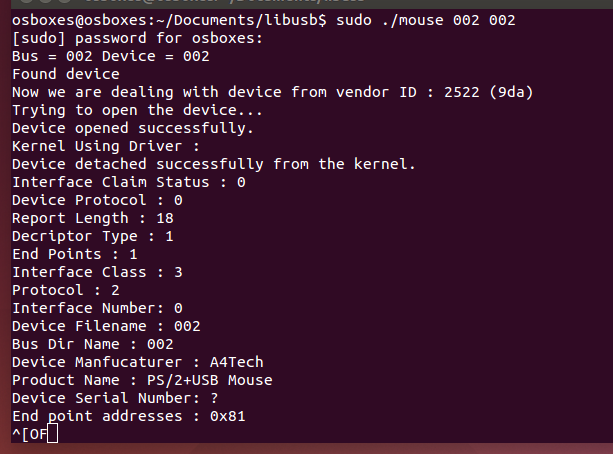
\includegraphics[width = \textwidth]{images/lol.png}}
  \caption{Информация об устройстве}
\end{figure}



\section{Вывод}
    В ходе выполнения курсовой работы был произведен анализ библиотеки libusb и написано тестовое приложение для взаимодействие с мышью. Приложение работает на операцонной системе Linux, так как именно на ней есть поддержка взаимодействия с HID устройствами. Также оно работает в пространстве пользователя, что отличает его от стандартного программного обеспечения - драйверов. Проведенный анализ библиотеки и опыт разработки на ней показал, что libusb обеспечиает достаточно легкий способ для взаимодейстия с usb устройствами.
\end{document}